\chapter{Introduction}
\section{Motivation}
Since the advent of Bitcoin, the groundbreaking peer-to-peer payment network and cryptocurrency, the ecosystem of blockchain technology has witnessed an exponential surge, propelling the emergence of numerous cryptocurrencies that are now widely utilized and traded. The soaring volatility of cryptocurrencies has not only captured the attention of retail investors, with some reaping substantial returns while others suffered significant losses~\cite{losing_money_on_crypto_2021}. Moreover, prominent financial institutions have joined the fray, aiming to capitalize on this novel tradable asset~\cite{gondek_what_nodate}. Consequently, this surge of interest has spurred the development of more sophisticated approaches to cryptocurrency trading.
\\[3mm]
Initially, trading cryptocurrencies posed a significant challenge for individuals lacking technical expertise, with the first recorded transaction occurring on $12^{th}$ October 2009 via a PayPal transaction~\cite{noauthor_history_nodate}. However, the landscape has since evolved, giving rise to various cryptocurrency exchanges, both centralised and decentralised. Centralised exchanges have gained popularity, offering a user-friendly interface and catering to investors with limited technical knowledge. In contrast, decentralised exchanges (DEXes) operate on blockchain networks and facilitate direct peer-to-peer transactions using smart contracts. The prevalence of centralised exchanges is evident, as depicted in Figure \ref{fig:dex_to_cex}, where the proportion of trades on DEXes remained minimal until the summer of 2020 but has been steadily increasing since then.

\begin{figure}[htb!]
    \centering
    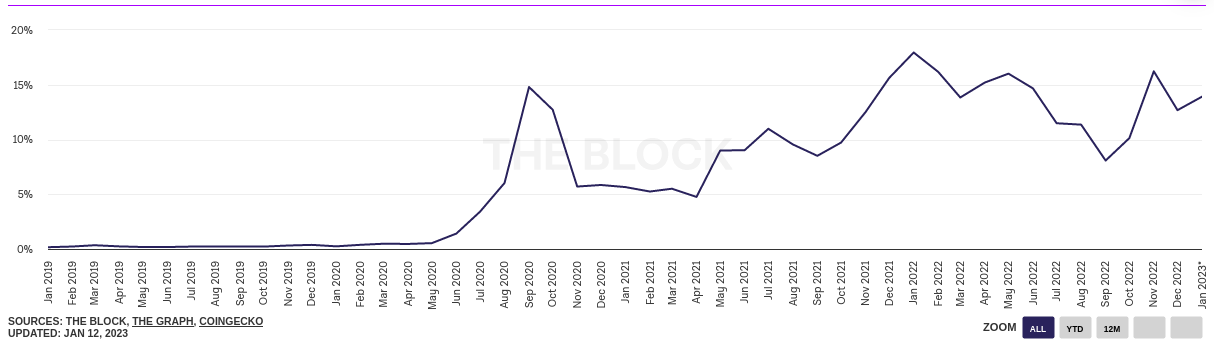
\includegraphics[width=\textwidth]{introduction/Images/dex_to_cex.png}
    \caption{{DEX} to {CEX} {Spot} {Trade} {Volume}~\cite{dex_to_cex}}
    \label{fig:dex_to_cex}
\end{figure}
\vspace{-1cm}
\section{Objectives}
This poses the question about which trading strategies can exploit arbitrage opportunities on decentralised exchanges. Although, there has been some research on this topic, focussing mainly on triangular and cyclic arbitrage on DEXes such as Uniswap and SushiSwap, however, there has been no research into analysing the performance of statistical arbitrage methods on decentralised exchanges. Therefore, this project aims to research methods of mean reversion in pairs trading of cryptocurrencies on decentralised exchanges.

\section{Contributions}
The work presented in the report is motivated by the rise in trading activity on decentralised exchanges. Exploring statistical arbitrage techniques on DEXes provides an opportunity to gain insights into the unique dynamics and potential profitability of decentralised markets. It allows traders to leverage their quantitative skills and exploit market inefficiencies to enhance trading performance and generate profits in the emerging landscape of decentralised finance. The contributions are as follows:
\begin{enumerate}[wide, labelwidth=!, labelindent=2ex]
    \itemsep-0.1em
    \item \textbf{Analysis of Liquidity Pool Pairs} - The analysis of liquidity pool pairs involves examining the correlation and cointegration between different pairs within a liquidity pool. This analysis provides insights into the pricing dynamics and long-term relationships that exist among the assets within the pool, hence exposing potential arbitrage opportunities. 
    \item \textbf{Backtesting System} - A meticulous backtesting system was developed to replicate the execution of trades by utilizing comprehensive historical data directly sourced from the Ethereum blockchain. This system enabled the evaluation of trading strategies under realistic and reliable market conditions, allowing for a thorough assessment of their performance.
    \item \textbf{Live Trading System} - To facilitate real-time trading and interaction with the Ethereum blockchain, a dynamic live trading system was designed and implemented. This system enabled the seamless execution of trading strategies in a live market environment.
    \item \textbf{Trading Strategies} - The mean reversion strategy relies on the hedge ratio, a key parameter that impacts the strategy's risk exposure and trading volumes. To assess the performance of different hedge ratio estimation methods, multiple strategies were employed: constant hedge ratio using ordinary least squares (OLS) as a benchmark, sliding window using OLS, lagged using OLS, Granger Causality test-based OLS model, and Kalman Filter-based hedge ratio estimation.
    \item \textbf{Novel Analysis of Applying Mean Reversion on Decentralised Exchanges}~- The analysis showed that the Kalman Filter strategy outperformed other mean reversion strategies and current research, achieving an Annual Percentage Return of 81.14\%. Equally noteworthy, the Granger Causality and Lagged strategies delivered substantial returns of 48.85\% and 38.70\% respectively, also surpassing returns observed in prior research on mean reversion and pure arbitrage across diverse asset classes.
\end{enumerate}

\section{Ethical Issues}

The ethics of cryptocurrencies are widely debated for reasons such as anonymity, leading it to be the choice of currency used by criminals and illegal institutions, volatility and lack of regulation. The high volatility makes cryptocurrencies and decentralised finance very risky for retail investors that don't have the technical or financial know-how making investing in cryptocurrencies.
\\[3mm]
Another aspect of cryptocurrencies that has raised ethical questions is the energy consumption and carbon dioxide emission from the mining of cryptocurrencies. Formal research about this has also been completed and found that `approximately 69 million metric tons of CO2 (Carbon dioxide) emission as a result of bitcoin mining'~\cite{egiyi2020cryptocurrency}. Thus, this is an ethical concern that I have thought about when designing the strategies so that the number of transactions that don't result in a profit, i.e. do not add value to the project, is limited.
\\[3mm]
In addition to the concerns above, although this project aims to find riskless profits, \textit{`free lunches'}, it is not, in any form, of financial advice, and those who use the research or software that used in the development and research process to attempt to get favourable results, are liable for the losses or gains. 
